\documentclass{exam}

\usepackage{graphicx}
\graphicspath{ {./images/} }

\usepackage{movie15}

\usepackage[T1]{fontenc}

\usepackage{hyperref}
\hypersetup{
    colorlinks=true,
    linkcolor=blue,
    filecolor=magenta,      
    urlcolor=blue,
    pdftitle={1XC3 Practice Exam Solutions},
    pdfpagemode=FullScreen,
    }
    
\usepackage{listings}
\usepackage{color}

\usepackage{amsmath}
\usepackage{amsfonts}
\usepackage{array}
\newcommand{\Mod}[1]{\ (\mathrm{mod}\ #1)}
\DeclareMathOperator{\lcm}{lcm}

\begin{document}
\lstset{frame=tb,
  language=c,
  aboveskip=5mm,
  belowskip=2mm,
  showstringspaces=false,
  columns=flexible,
  basicstyle={\small\ttfamily},
  numbers=none,
  numberstyle=\tiny\color{blue},
  keywordstyle=\color{red},
  commentstyle=\color{pink},
  stringstyle=\color{green},
  breaklines=true,
  breakatwhitespace=true,
  tabsize=4}


\begin{center}\noindent\rule{6in}{0.4pt}\end{center}

Name : \underline{\hspace{2.5in}} Student No. : \underline{\hspace{2in}}

\begin{center}
\fbox{

\fbox{\parbox{5.5in}{\centering
\textbf{COMPSCI 1XC3 PRACTICE EXAM - SOLUTIONS}\\[0pt]
April 12\textsuperscript{\textit{th}}, 2023\\
Instructor: Richie Motorgeanu (totally)\\
Duration: 150 minutes
}}

}

\vspace{20px}

\begin{tabular}{ | c | c | } 
  \hline
  Start Time & whatever time it is now \\ 
  \hline
  End Time & whatever time it is 150 minutes from now \\ 
  \hline
\end{tabular}

\vspace{10px}

\textbf{YOU ARE RESPONSIBLE FOR ENSURING THAT YOUR COPY OF THE PAPER IS COMPLETE. BRING ANY DISCREPANCY TO THE ATTENTION OF YOUR INVIGILATOR.}
\end{center}

\vspace{10px}

\textbf{Materials Permitted In The Exam Venue:}

\textbf{(No electronic aids are permitted e.g. laptops, phones)}

One Double Sided 8.5 x 11 Crib Sheet

Calculator

\vspace {70px}

\begin{center}

\Large \begin{tabular}{ || c || c || } 
  \hline
  Section & Points \\ 
  \hline
  Section 1 &   /30 \\ 
  \hline
  Section 2 &   /25 \\ 
  \hline
  Section 3 &   /53 \\ 
  \hline
  Total &   /100 \\ 
  \hline
\end{tabular}

\end{center}

\newpage

%----------------------------------------------------------------------------------------

%	PAGE 1

%----------------------------------------------------------------------------------------

\begin{center}\noindent\rule{6in}{0.4pt}\end{center}

{\Large\textbf{Section 1: multiple-choice questions (30 points)}}
\\

% QUESTION 1
\textbf{Question 1} (3 points) Given the following lines of code, what addresses will the pointers be pointing to?

\begin{lstlisting}
int* ptr1= 0x7fff98ef9170;
void* ptr2 = 0x7fff98ef9170;
ptr1 += 1;
ptr2 += 1;
\end{lstlisting}

\begin{center}

\begin{tabular} { c  c } 
  A. ptr1: 0x7fff98ef9174, ptr2: 0x7fff98ef9174 & B. ptr1: 0x7fff98ef9171 ptr2: 0x7fff98ef9171 \\ 

  C. ptr1: 0x7fff98ef9171 ptr2: 0x7fff98ef9174 & \textbf{D. ptr1: 0x7fff98ef9174 ptr2: 0x7fff98ef9171}
\end{tabular}

\vspace{5px}
\textcolor{blue}{Adding 1 to an integer pointer will add 1 * sizeof(int). Adding 1 to a void pointer will literally add 1 to it.}

\end{center}

\vspace{10px}

% QUESTION 2
\textbf{Question 2} (3 points) A struct can contain an instance of itself.

\begin{center}

\begin{tabular} { c  c } 
  A. True & \textbf{B. False} \\ 
\end{tabular}

\vspace{5px}
\textcolor{blue}{A struct can however contain a pointer to an instance of itself.}

\end{center}

% QUESTION 3
\textbf{Question 3} (3 points) Consider the following files. What would be outputted if we used the “diff” command on the two of them?

\begin{center}
\begin{tabular} { | m{1in} | m{1in} | } 
WIDTH=1920 \newline HEIGHT=1080 \newline MONITORS=2
& 
WIDTH=1920 \newline HEIGHT=1080 \newline MONITORS=3
\end{tabular}
\end{center}

\begin{center}

\begin{tabular} { p{3in}  p{3in} } 
  A.  No output. & \textbf{B. \newline 3c3 \newline < MONITORS=2 \newline --- \newline > MONITORS=3 \newline}\\

  C.  \newline < MONITORS=2 \newline --- \newline > MONITORS=3 & D. \newline WIDTH=1920 \newline HEIGHT=1080 \newline < MONITORS=2 \newline --- \newline > MONITORS=3 \\
\end{tabular}

\end{center}

\vspace{10px}

% QUESTION 4
\textbf{Question 4} (3 points) Given the following lines of code, pick the most correct answer.

\begin{center}
i) sizeof(int*);\\
ii) sizeof(float*);\\
iii) sizeof(int**);\\
\end{center}

\begin{center}

\begin{tabular} { c  c } 
  \textbf{A. i), ii), and iii) would compile successfully and return the same values.}\\
  B. i), ii), and iii) would compile successfully but return different values. \\ 
  C. i) and ii) would compile successfully and return the same values, but iii) would not compile. \\ 
  D. i) and ii) would compile successfully but return different values, and iii) would not compile.
\end{tabular}

\end{center}

\vspace{10px}

\newpage

%----------------------------------------------------------------------------------------

%	PAGE 2

%----------------------------------------------------------------------------------------

\begin{center}\noindent\rule{6in}{0.4pt}\end{center}

% QUESTION 5
\textbf{Question 5} (3 points) Suppose you have a pointer to a struct. Which of the following are valid ways of accessing a struct’s field using the pointer?

\begin{center}

\begin{tabular} { c  c } 
  A. ptrStruct -> myField &
  B. (*ptrStruct).myField \\ 
  \textbf{C. A and B} &
  D. None of the above.
\end{tabular}

\end{center}

\vspace{10px}

% QUESTION 6
\textbf{Question 6} (3 points) What does the following line of code do?

\begin{center}
cat notes.txt | head -3 | tail -3
\end{center}

\begin{center}

\begin{tabular} { c  c } 
  \textbf{A. Retrieves the first three lines of “notes.txt”}\\
  B. Retrieves the last three lines of “notes.txt” \\ 
  C. Retrieves the first three lines and the last three lines of “notes.txt” \\ 
  D. Retrieves all the lines except the first three lines and the last three lines of “notes.txt"
\end{tabular}

\end{center}

\vspace{10px}

% QUESTION 7
\textbf{Question 7} (3 points) What does calloc() do?

\begin{center}

\begin{tabular} { c  c } 
  A. It deallocates a chunk of memory. \\
  B. It allocates n chunks of memory and overwrites previous data with a specified value. \\ 
  \textbf{C. It allocates n chunks of memory and overwrites previous data with “0”s. }\\
  D. It changes the amount of memory allocated to a pointer.
\end{tabular}

\end{center}

\vspace{10px}

% QUESTION 8
\textbf{Question 8} (3 points) Which of the following statements are correct?

\begin{center}

\begin{tabular} { c  c } 
  A. An uninitialized pointer will point to a random location of valid memory. \\
  \textbf{B. An uninitialized pointer will point to a random location of potentially valid memory. }\\
  C. An uninitialized pointer will point to null. \\ 
  D. The usage of an uninitialized pointer is guaranteed to cause a runtime error.
\end{tabular}

\end{center}

\vspace{10px}

% QUESTION 9
\textbf{Question 9} (3 points) What should you not do when documenting your code?

\begin{center}

\begin{tabular} { c  c } 
  A. Explain how it works. &
  B. Use self-documenting variable names. \\ 
  \textbf{C. Comment everything. }&
  D. Document the purpose of the file.
\end{tabular}

\vspace{5px}
\textcolor{blue}{Don't overcomment! Only commend necessary things, like the tops of functions or important blocks of code.}

\end{center}

\vspace{10px}

% QUESTION 10
\textbf{Question 10} (3 points) Given the following line of code, which of these is not a valid way to get the address of the first element in an array?

\begin{center}
int arr[5] = \{1,2,3,4,5\};
\end{center}

\begin{center}

\begin{tabular} { c c c c } 
  A. arr &
  B. \text{\&arr} &
  C. \text{\&arr[0]} &
  \textbf{D. None of the above.}
\end{tabular}

\end{center}

\vspace{10px}

\newpage

%----------------------------------------------------------------------------------------

%	PAGE 3

%----------------------------------------------------------------------------------------

\begin{center}\noindent\rule{6in}{0.4pt}\end{center}

{\Large\textbf{Section 2: program segment questions (25 points)}}
\\

% QUESTION 11
\textbf{Question 11} (5 points) The output of the following shell script is:

\lstset{frame=tb,
  language=bash,
  aboveskip=5mm,
  belowskip=2mm,
  showstringspaces=false,
  columns=flexible,
  basicstyle={\small\ttfamily},
  numbers=none,
  numberstyle=\tiny\color{blue},
  keywordstyle=\color{red},
  commentstyle=\color{magenta},
  stringstyle=\color{blue},
  breaklines=true,
  breakatwhitespace=true,
  tabsize=4}
\begin{lstlisting}
a=0

while [ "$a" -lt 10 ]
do
    b=$a
    
    if [ "$b" -ge 3 ]; then
        echo -e $b hello >> temp.txt
    else
        echo hello $a > temp.txt
    fi

    a=$(($a+1))

done
    
# tac reverses order of lines (tac is cat spelt backwards)
cat temp.txt | head -5 | tac
\end{lstlisting}
\lstset{frame=tb,
  language=c,
  aboveskip=5mm,
  belowskip=2mm,
  showstringspaces=false,
  columns=flexible,
  basicstyle={\small\ttfamily},
  numbers=none,
  numberstyle=\tiny\color{blue},
  keywordstyle=\color{red},
  commentstyle=\color{magenta},
  stringstyle=\color{blue},
  breaklines=true,
  breakatwhitespace=true,
  tabsize=4}

\textbf{Answer:}

6 hello

5 hello

4 hello

3 hello

hello 2

\newpage



%----------------------------------------------------------------------------------------

%	PAGE 5

%----------------------------------------------------------------------------------------

\begin{center}\noindent\rule{6in}{0.4pt}\end{center}

% QUESTION 12
\textbf{Question 12} (5 points) The output of the following C program segment is:

\begin{lstlisting}
int main(void) {
  int *i, s[4], t[4], *u = s;
  
  for (i = s; i - s <= 3; i++) 
  {
    *i = i - s;
    *(t + *(i)) = 2* *(s + *(i));
  }
  
  printf("s:t\n");
  
  for (i = s; i-s <= 3; i++) 
    printf("%d:%d\n", *(s + *i), *(t + *i));
    
  printf("u = %d\n", *u);
}
\end{lstlisting}

\textbf{Answer:}

s:t

0:0

1:2

2:4

3:6

u = 0

\newpage

%----------------------------------------------------------------------------------------

%	PAGE 6

%----------------------------------------------------------------------------------------

\begin{center}\noindent\rule{6in}{0.4pt}\end{center}

% QUESTION 13
\textbf{Question 13} (5 points) The output of the following C program segment is:

\begin{lstlisting}
// Implementation of Queue is not shown. Behaves like a Queue data type.
// queue(int, *Queue): adds an integer to the Queue
// dequeue(*Queue): removes the next integer from the Queue. returns the removed integer.

// Implementation of Stack is not shown. Behaves like a Stack data type.
// push(int, *Stack): adds an integer to the Stack
// pop(*Stack): removes the next integer from the Stack. returns the removed integer.

int main(void) {
    Queue q;  // Creates an empty queue of integers
    Stack s; // Creates an empty stack of integers.
    
    for(int i = 0; i < 10; i++) {
        queue(i*2, &q);
        push(i*2+1, &s); 
    }
 
    for(int i = 0; i < 10; i++) {
    	printf("%d:", dequeue(&q));
    	printf("%d\n", pop(&p));
    }
}
\end{lstlisting}

\textbf{Answer:}

0:19

2:17

4:15

6:13

8:11

10:9

12:7

14:5

16:3

18:1


\newpage

%----------------------------------------------------------------------------------------

%	PAGE 7

%----------------------------------------------------------------------------------------

\begin{center}\noindent\rule{6in}{0.4pt}\end{center}

% QUESTION 14
\textbf{Question 14} (5 points) The output of the following C program segment is:

\begin{lstlisting}

int myFunc(int a, int *b, int *c, int d) {
	a = *b;
	*b = *c;
	*c = d;
	d = a;
	return (a * *c) + (*b * d);
}

int main(void) {
	int w = -2;	
	int x = 5;
	int y = 3;
	int z = 6;
	
	int f = myFunc(w, &y, &x, z);
	
	printf("%d, %d, %d, %d, %d", w, x, z, f, y);
}

\end{lstlisting}

\textbf{Answer:}

-2, 6, 6, 33, 5

\newpage

%----------------------------------------------------------------------------------------

%	PAGE 8

%----------------------------------------------------------------------------------------

\begin{center}\noindent\rule{6in}{0.4pt}\end{center}

% QUESTION 15
\textbf{Question 15} (5 points) The output of the following C program segment is:

\begin{lstlisting}

int main(void) {
	int num = 255;
	
	printf("%d\n", num);
	printf("%i\n", num);
	printf("%o\n", num);
	printf("%x\n", num);
	printf("%X\n", num);
	
	printf("%5d\n", num);
	printf("%4d\n", num);
	printf("%3d\n", num);
	printf("%2d\n", num);
	printf("%1d\n", num);
	
	printf("%.5d\n", num);
	printf("%.3d\n", num);
	printf("%.1d\n", num);
}

\end{lstlisting}

\textbf{Answer:}

255

255

377

ff

FF

\hspace{10px}255
  
\hspace{5px}255
 
255

255

255

00255

255

255


\newpage

%----------------------------------------------------------------------------------------

%	PAGE 9

%----------------------------------------------------------------------------------------

\begin{center}\noindent\rule{6in}{0.4pt}\end{center}

{\Large\textbf{Section 3: coding (53 points)}}
\\

% QUESTION 16
\textbf{Question 16} (8 points) Please write a shell script that does the following.

i) Creates an empty file "myCollection.txt" if it doesn't exist.

ii) Give all files in the current directory executable permissions.

iii) Appends lines 3-7 of "main.bash" to "myCollection.txt"

You can assume that the current directory contains only files. 

\textbf{Answer:}

\lstset{frame=tb,
  language=bash,
  aboveskip=5mm,
  belowskip=2mm,
  showstringspaces=false,
  columns=flexible,
  basicstyle={\small\ttfamily},
  numbers=none,
  numberstyle=\tiny\color{blue},
  keywordstyle=\color{red},
  commentstyle=\color{magenta},
  stringstyle=\color{blue},
  breaklines=true,
  breakatwhitespace=true,
  tabsize=4}
\begin{lstlisting}
if ! [ -f "myCollection.txt" ]; then
    touch myCollection.txt
fi

ls | xargs chmod +x 

cat main.bash | head -7 | tail -5 | xargs -i echo {} >> "myCollection.txt" 
\end{lstlisting}
\lstset{frame=tb,
  language=c,
  aboveskip=5mm,
  belowskip=2mm,
  showstringspaces=false,
  columns=flexible,
  basicstyle={\small\ttfamily},
  numbers=none,
  numberstyle=\tiny\color{blue},
  keywordstyle=\color{red},
  commentstyle=\color{magenta},
  stringstyle=\color{blue},
  breaklines=true,
  breakatwhitespace=true,
  tabsize=4}

\textcolor{blue}{This won't produce perfect results (it ignores empty lines), but you'll get full marks if I were the prof}

\newpage

%----------------------------------------------------------------------------------------

%	PAGE 10

%----------------------------------------------------------------------------------------

\begin{center}\noindent\rule{6in}{0.4pt}\end{center}

% QUESTION 17
\textbf{Question 17} (12 points) Write a C program that reads the content of "myCollection.txt" and copies all lowercase vowel characters over to "yoeioo.txt".

You can assume that the files already exist. Include y in the vowels.

\textbf{Answer:}

\begin{lstlisting}
#include <stdio.h>

int main(void) {
	FILE *inputFile = fopen("myCollection.txt", "r");
	FILE *outputFile = fopen("yoeioo.txt", "w");

	char t;
	
	while(fscanf(inputFile, "%c", &t) == 1) {
		if(t == 'a' || t == 'e' || t == 'i' || t == 'o' || t == 'u' || t == 'y') {
			fprintf(outputFile, "%c", t);
		}
	}

	fclose(inputFile);
	fclose(outputFile);
}
\end{lstlisting}

\newpage

%----------------------------------------------------------------------------------------

%	PAGE 11

%----------------------------------------------------------------------------------------

\begin{center}\noindent\rule{6in}{0.4pt}\end{center}

% QUESTION 18
\textbf{Question 18} (15 points) Given the root of a binary tree of integers, write a function that finds the sum of all nodes in the tree.

\begin{lstlisting}
struct BinTree {
	int value;
	struct BinTree *left;
	struct BinTree *right;
};
\end{lstlisting}

\textbf{Tree Summing Algorithm.} The basic steps to perform Tree Summation are:

1) If the left tree doesn't exist (i.e, is a null pointer), its sum is zero. Move on to step 3.

2) If the left tree exists, we recursively call the summing function on the left tree.

3) If the right tree doesn't exist (i.e, is a null pointer), its sum is zero. Move on to step 5.

4) If the right tree exists, we recursively call the summing function on the right tree.

5) Add up the sum of the left tree, right tree, and the value of the current Node and return this value.

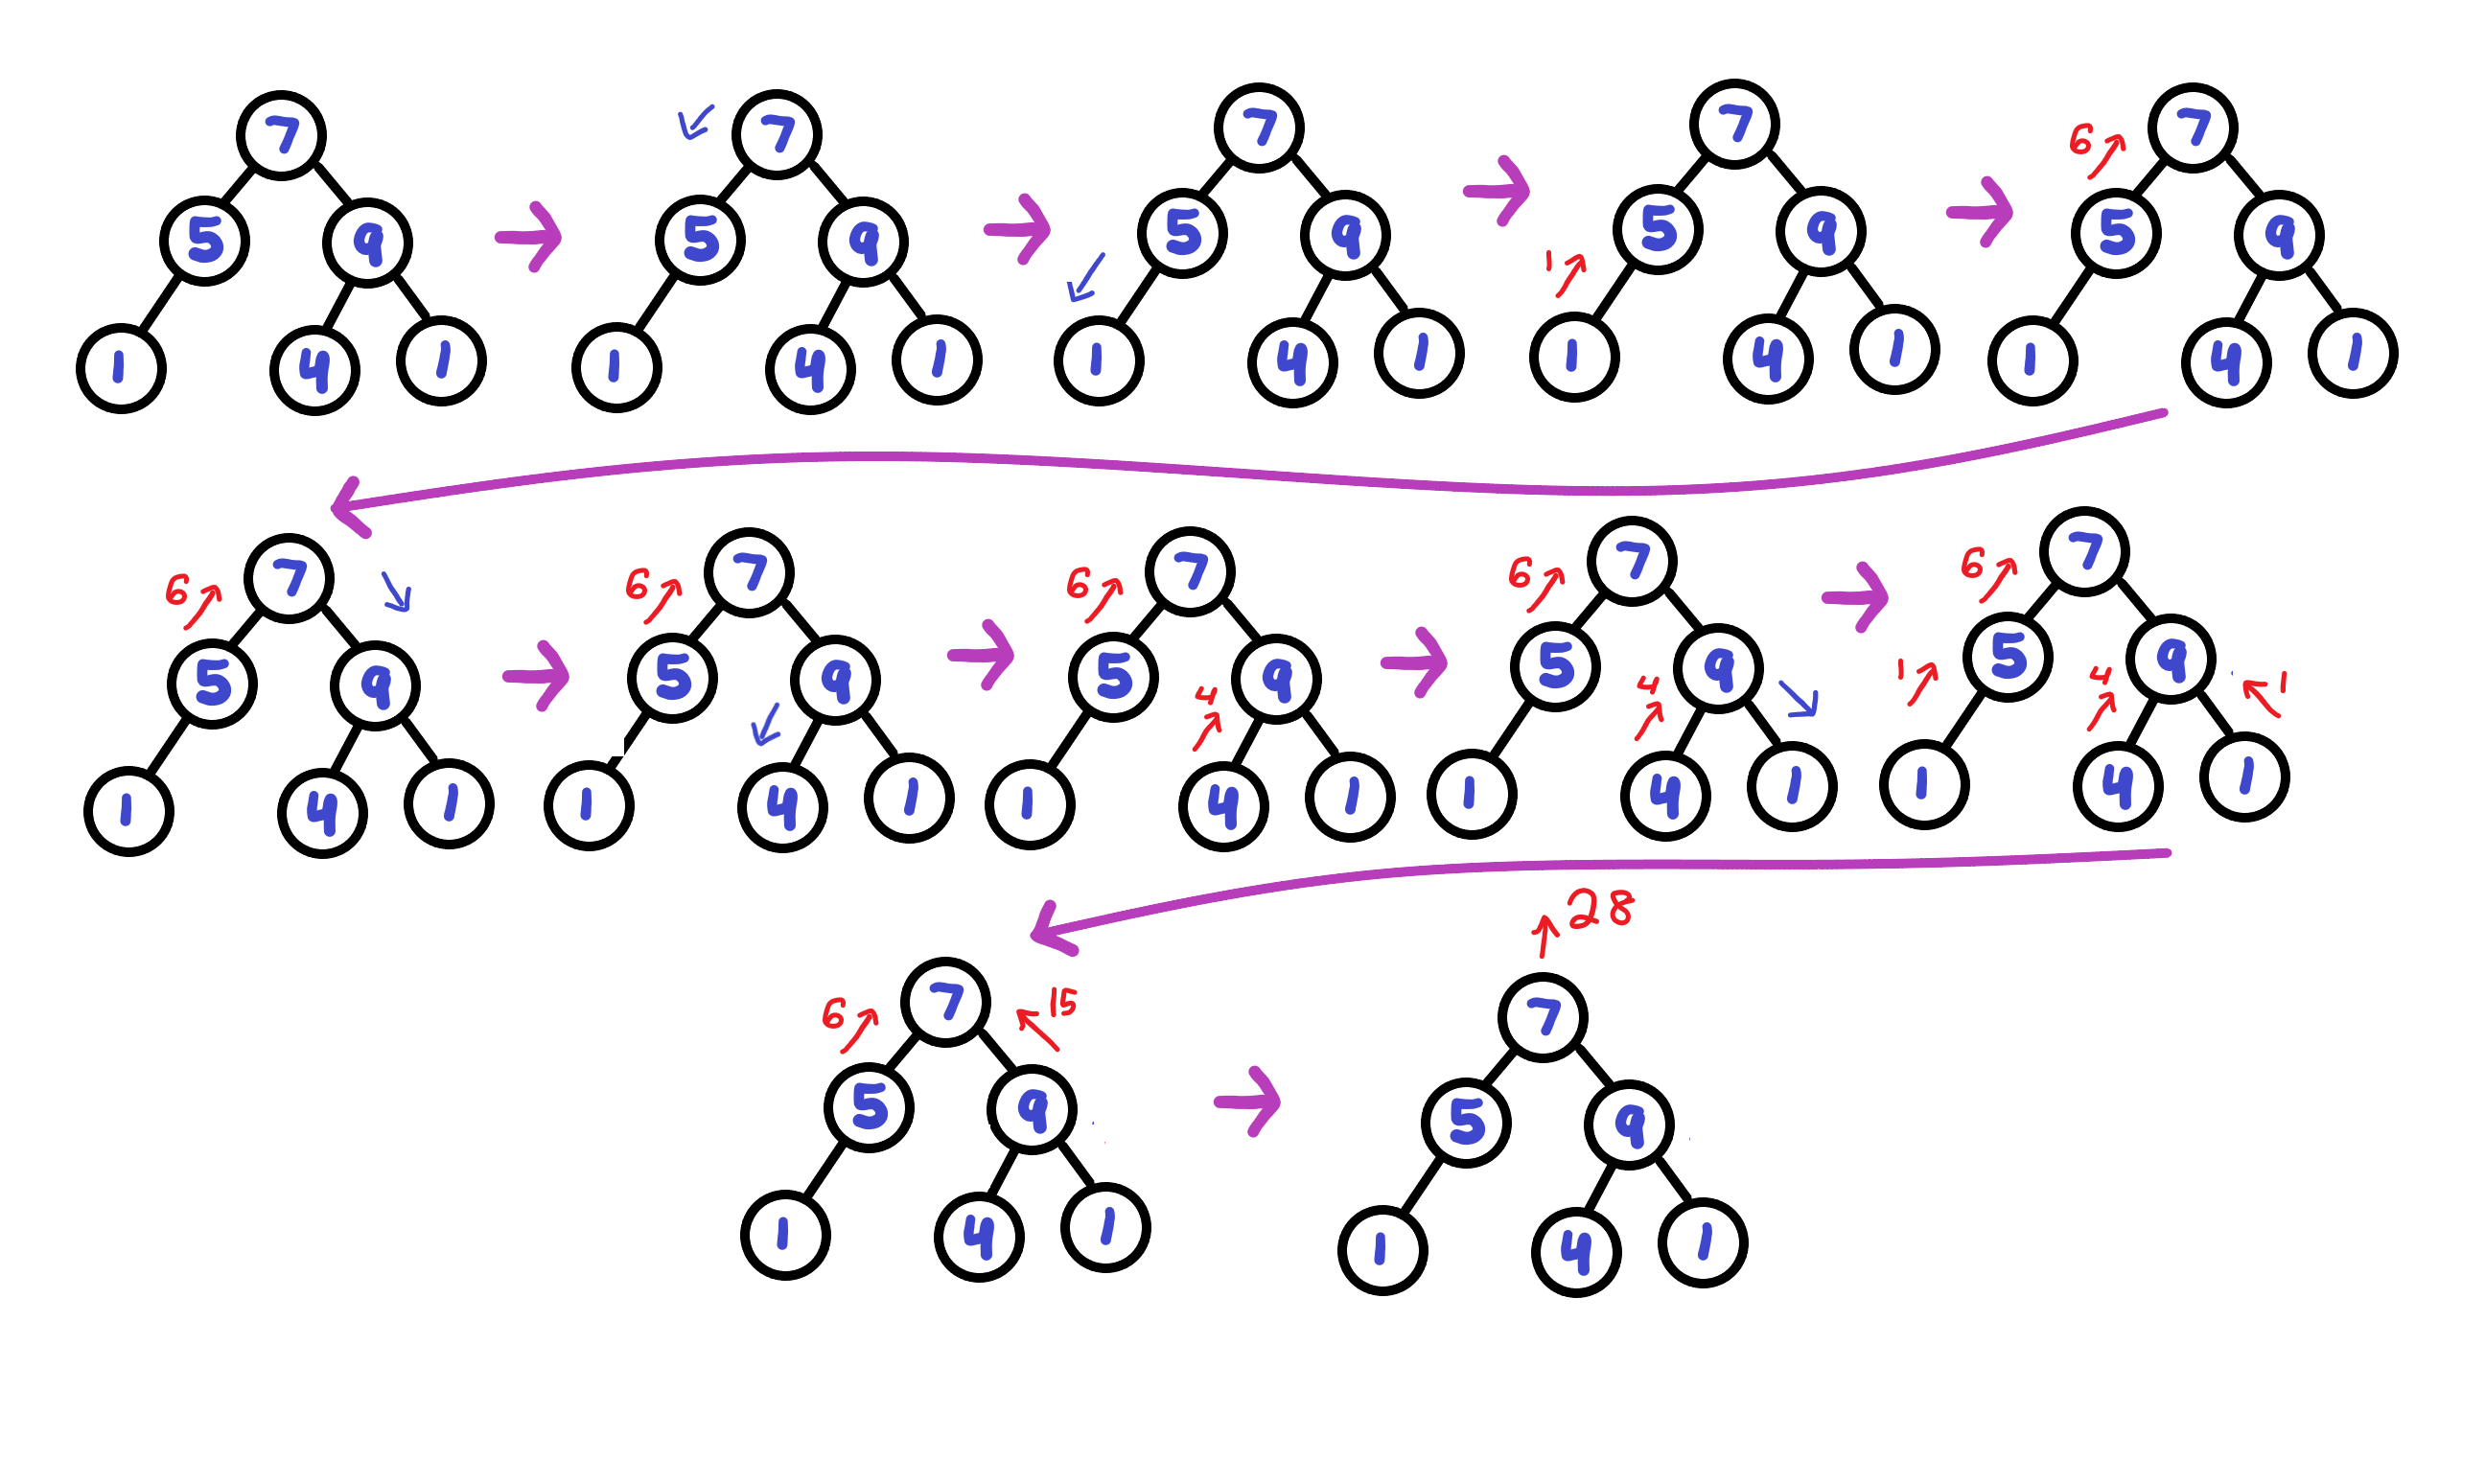
\includegraphics[scale=0.15]{tree}

\textbf{Answer:}

\begin{lstlisting}
typedef struct BinTree bintree;
int treeSum(bintree root) {

	int leftSum = 0;
	int rightSum = 0;

	if(root.left != 0) {
		leftSum = treeSum(*root.left);
	}

	if(root.right != 0) {
		rightSum = treeSum(*root.right);
	}
	
	return root.value + leftSum + rightSum;
}
\end{lstlisting}

\newpage

%----------------------------------------------------------------------------------------

%	PAGE 12

%----------------------------------------------------------------------------------------

\begin{center}\noindent\rule{6in}{0.4pt}\end{center}

% QUESTION 19
\textbf{Question 19} (18 points) There are two parts to this question. Part 1 is 10 points, Part 2 is 8 points.

i) Create a struct for a Singly-Linked List named "Student". It should store an integer field named "debt". Suppose you have a pointer "head" that points to the head of a linked list. Create a function "frontInsert" that takes in a pointer to the head pointer and an integer "newDebt". The function should create a new Student with "newDebt" debt and set that to be the new head of the linked list.

ii) Create a function "reverseList" that takes in a pointer to the head pointer. The function should reverse the order of the linked list, so that the end of the linked list becomes the new head.

\textbf{Answer:}

\begin{lstlisting}
typedef struct Student student;

struct Student {
	int debt;
	student *next;
};

void frontInsert(student **head, int newDebt) {
	student *newStudent = malloc(sizeof(student));
	newStudent -> next = *head;
	newStudent -> debt = newDebt;
	*head = newStudent;
}

void reverse(student **head) {
	student *previous = 0;
	student *current = *head;
	student *next = *head;
	
	while(next != 0) {
		next = current -> next;
		current -> next = previous;
		previous = current;
		current = next;
	}

	*head = previous;
}
\end{lstlisting}

\textcolor{blue}{Note: A variable declared within a function will \textbf{disappear} after the function returns. By using malloc, we allocate the neccessary memory to allow newStudent to persist after the function returns. LMK if I'm just being dumb and I'll update the solution.}

\textcolor{blue}{\href{https://www.geeksforgeeks.org/reverse-a-linked-list/}{\underline{Here}} is a wonderful resource that helps explain the reversing of a linked list.}

\newpage

\begin{center}\noindent\rule{6in}{0.4pt}\end{center}

\newpage

\begin{center}\noindent\rule{6in}{0.4pt}\end{center}

\begin{center}\noindent\rule{6in}{0.4pt}\end{center}

\vspace{5px}

\begin{center} END OF EXAM \end{center}

\end{document}